\documentclass[9pt]{sigplanconf}
\usepackage{url}
\usepackage{tikz}
\usepackage{graphicx}
\usepackage{framed}
\usepackage{color}
\usepackage{url}
\usepackage{alltt}
\usepackage{tabularx}
\usepackage{subfigure}
\usepackage{fancyhdr}
\usepackage{paralist}

\usepackage{pgf}
\usepackage{tikz}
\usetikzlibrary{arrows,automata}

%% \include{math}


%% \newenvironment{code}{\begin{framed}\begin{alltt}\scriptsize}{\end{alltt}
%%   \end{framed}}
\newenvironment{code}{\begin{alltt}\footnotesize}{\end{alltt}}
\newenvironment{cols}{\begin{tabular}{m{3.6cm}|m{3.6cm}}{Haskell} &
    {\scriptsize Copilot}\\\hline}{\end{tabular}}

\usepackage{ifthen}
\newboolean{submission}  %set to true for the submission version
%\setboolean{submission}{false}
\setboolean{submission}{true}
\ifthenelse
{\boolean{submission}}
{ \newcommand{\todo}[1]{ } } %hide todo
{ \newcommand{\todo}[1]{ {\color{blue}$<<$#1$>>$}
 }}
%\usepackage{fancyhdr}


\begin{document}

\conferenceinfo{ICFP'12,} {September 9--15, 2012, Copenhagen, Denmark.}
\CopyrightYear{2012}
\copyrightdata{978-1-4503-1054-3/12/09}

%\titlebanner{banner above paper title}        % These are ignored unless
%\preprintfooter{}   % 'preprint' option specified.

\title{Experience Report: a Do-It-Yourself High-Assurance Compiler}
%\subtitle{Subtitle Text, if any}

\authorinfo{Lee Pike}
           {Galois, Inc.}
           {leepike@galois.com}
\authorinfo{Nis Wegmann}
           {University of Copenhagen}{niswegmann@gmail.com}
\authorinfo{Sebastian Niller}
           {Unaffiliated}{sebastian.niller@gmail.com}
\authorinfo{Alwyn Goodloe}
           {NASA}{a.goodloe@nasa.gov}
\maketitle

\begin{abstract}
Embedded domain-specific languages (EDSLs) are an approach for quickly building
new languages while maintaining the advantages of a rich metalanguage.  We argue
in this experience report that the ``EDSL approach'' can surprisingly ease the
task of building a high-assurance compiler.  We do not strive to build a fully
formally-verified tool-chain, but take a ``do-it-yourself'' approach to increase
our confidence in compiler-correctness without too much effort.  \emph{Copilot}
is an EDSL developed by Galois, Inc. and the National Institute of Aerospace
under contract to NASA for the purpose of runtime monitoring of flight-critical
avionics.  We report our experience in using type-checking, QuickCheck, and
model-checking ``off-the-shelf'' to quickly increase confidence in our EDSL
tool-chain.
\end{abstract}

\category{D.2.4}{Software/Program Verification}{Reliability}

\terms
Languages, Verification

\keywords
embedded domain-specific language, compiler, verification


%\todo{emails for sebastian, nis?}

%% \institute{Galois, Inc. \email{leepike@galois.com}
%% \and National Institute of Aerospace \email{sebastian.niller@nianet.org}
%% \and University of Copenhagen \email{wegmann@diku.dk}
%% %\and NASA Langley Research Center \email{a.goodloe@nasa.gov}
%% }


\section{Introduction}\label{sec:intro}

%% cite Filet-o-Fish: practical and dependable domain-specific languages https://personal.cis.strath.ac.uk/pierreevariste.dagand/}

The ``do-it-yourself'' (DIY) culture encourages individuals to design and craft
objects on their own, without relying on outside experts.  DIY construction
should be inexpensive with easy-to-access materials.  Ranging from hobbyist
electronics\footnote{This even includes full-featured unpiloted air vehicles!
  See \url{http://diydrones.com/}.} to urban farming to fashion, DIY is making
somewhat of a resurgence across the United States.

We see no reason why DIY culture should not also extend to compilers, and in
particular, to high-assurance compilers.  By \emph{high-assurance}, we mean a
compiler that comes with compelling evidence that the source code and object
code have the same operational semantics.

High-assurance compilers development has traditionally required years of effort
by experts.  A notable early effort was the CLI Stack, of which a simple
verified compiler was one part~\cite{cli}.  The CLI Stack was verified by the
precursor to the ACL2 theorem prover.  The most recent instance is CompCert,
which compiles a subset of C suitable for embedded development to machine code
for a number of targets~\cite{leroy}.  CompCert is formally verified in the Coq
theorem-prover---indeed, CompCert is written in Coq's specification language.
While CompCert achieves the highest levels of assurance, generating the evidence
comes at a steep price, since it relies on manually interacting with a
theorem-prover.  Neither the CLI Stack nor CompCert are DIY projects:
building them requires relatively esoteric skills that combine interactive
theorem-proving and multiple engineer-years of verification effort.

In this experience report, we argue that by leveraging functional languages and
off-the-shelf verification tools, we can accumulate significant evidence of
correctness at a fraction of the cost and without the specialized know-how
required by interactive verification approaches.  

The case-study of our approach is the Copilot language and toolset, developed by
Galois, Inc. and the National Institute of Aerospace under contract to NASA.
Copilot is a stream language for generating embedded C-code software monitors
for system properties.  Copilot itself is not comparable to a verified compiler
like CompCert: Copilot back-ends stop at the C level, where CompCert starts.
Verifying C semantics against the semantics of a machine model is
extraordinarily difficult.  Still, for high-level languages, we can do much
better than the status quo.

Specifically, we employ three not-so-secret weapons from the functional languages
and formal methods communities in our work.
\begin{compactenum}
\item {\em Embedded DSLs}: We implement Copilot as an embedded domain-specific
  (EDSL) language~\cite{meijer} within Haskell.
\item {\em Sub-Turing complete languages}: Copilot is targeted at embedded
  programming, therefore we focus on the class of programs that are computable
  in constant time and constant space.
\item {\em A verifying compiler}: CompCert typifies a \emph{verified compiler}
  approach in which the compiler itself is proved correct.  A \emph{verifying
    compiler} is one that provides evidence that a specific compilation is
  correct~\cite{mcrypt}.  We borrow from this second approach.  (We emphasize
  that this report is about assurance of the EDSL compiler itself, not about the
  functional correctness of programs written in the EDSL.)
\end{compactenum}

\noindent
While the approaches we describe are known within the functional programming and
formal methods communities, the purpose of this experience report is to
demonstrate the engineering ease in putting them to use.  In particular, the
EDSL approach is well-known for quickly prototyping new languages, but the reader
should have some level of skepticism that they are appropriate for
high-assurance development; we hope to dispel that skepticism.  Furthermore,
there is nothing special about the Copilot language with respect to assurance.
We hope to convince the reader that the approach we have taken can be applied
broadly to new language design.

\paragraph{Outline.}
In Section~\ref{sec:copilot}, we briefly introduce Copilot (we assume some
familiarity with Haskell syntax).  The heart of the report is
Section~\ref{sec:lessons} in which we describe our ``lessons learned'' for
easily generating evidence of correctness.  We briefly mention related work in
Section~\ref{sec:related}, and make concluding remarks in
Section~\ref{sec:conclusions}.


%--------------------------------------------------------------------------------
\section{The Copilot Language \& Toolset}\label{sec:copilot}
From 2009-2011, NASA contracted Galois, Inc. to research the possibility of
augmenting complex aerospace software systems with \emph{runtime verification}
(RV).  RV is a family of approaches that employ \emph{monitors} to observe the
behavior of an executing system and to detect if it is consistent with a formal
specification.  A monitor implementation should be simple and direct and serve
as the last line of defense for the correctness for the system.  The need for
aerospace RV is motivated by recent failures in commercial avionics and the
space shuttle~\cite{monitors}.

Our answer to the contract goals was Copilot, an EDSL to generate embedded
monitors.\footnote{Copilot source code is available at
  \url{http://leepike.github.com/Copilot/} and is licensed under the BSD3
  license.}  The Copilot language itself, focusing on its RV uses for NASA, has
been previously described~\cite{pike-rv-11}.  We will very briefly introduce
Copilot in this paper; our focus is more specifically about compiler
correctness.

One research challenge of the project was phrased as, ``Who watches the
watchmen?'' meaning that if the RV monitor is the last line of defense, then it
must not fail or worse, introduce unintended faults itself!  Nonetheless,
because the primary goal of the project was to implement an RV system and to
field-test it, few resources were available for assuring the correctness of the
Copilot compiler.  Our approach was born out of necessity.



%% Copilot currently includes a pretty-printer, an interpreter, two compilers
%% generating embedded C code, and a model-checker interface.  We describe our use
%% of the tools with respect to evidence generation in the following section.

\paragraph{Copilot's expression language.}
In the following, we briefly and informally introduce Copilot's expression
language.  One design goal for Copilot is to use a familiar syntax and model of
computation; doing so is a first step in reducing specification errors.  The
Copilot language mimics both the syntax and semantics of lazy lists (which we
call \emph{streams}) in Haskell.  One notable exception though is that
operators are automatically promoted point-wise to the list level, much like in
Lustre, a declarative language for embedded programming~\cite{lustre}.  For
example, the Fibonacci sequence modulo $2^{32}$ can be written as follows in Haskell:
%
\begin{code}
fib :: [Word32]
fib = [0,1] ++ zipWith (+) fib (drop 1 fib)
\end{code}
%
In Copilot, the equivalent definition is the following:
\begin{code}
fib :: Stream Word32
fib = [0,1] ++ (fib + drop 1 fib)
\end{code}
%
Copilot overloads or redefines many standard operators from Haskell's Prelude
Library.  Here is a Haskell and equivalent Copilot function that implements a
latch (flip-flop) over streams---the output is the XOR of the input stream and
the latch's previous output.  For example, for the input stream
%
\begin{code}
T, F, F, T, F, F, T, F, F, ...
\end{code}
%
{\tt latch} generates the stream
\begin{code}
F, T, T, T, F, F, F, T, T, T, ...
\end{code}
%
In Haskell, {\tt latch} can be defined
\begin{code}
latch :: [Bool] -> [Bool]
latch x = out x
  where 
  out ls   = [False] ++ zipWith xor ls (out ls)
  xor n m  = (n || m) && not (n && m)
\end{code}
%
and then in Copilot ({\tt xor} is a built-in operator for Copilot):
%
\begin{code}
latch :: Stream Bool -> Stream Bool
latch x = out
  where out = [False] ++ x `xor` out
\end{code}
% 
The base types of Copilot over which streams are built include Booleans, signed
and unsigned words of 8, 16, 32, and 64 bits, floats, and doubles. Type-safe
casts in which overflow cannot occur are permitted.

\paragraph{Sampling.}
Copilot programs are meant to monitor arbitrary C~programs.  They do so by
periodically \emph{sampling} symbol values. (Copilot samples variables, arrays,
and the return values of side-effect free functions---sampling arbitrary
structures is future work.)  For a Copilot program compiled to~C, symbols become
in-scope when arbitrary C~code is linked with the code generated by the Copilot
compiler.  Copilot provides the operator {\tt extern} to introduce an external
symbol to sample.  The operator types a string denoting the C~symbol.

Copilot can be interpreted as well as compiled.  When interpreted,
representative values are expected to be supplied by the programmer.  For
example, the following stream samples the C variable {\tt e0} of type {\tt
  uint8\_t} to create each new stream index.  If {\tt e0} takes the values {\tt
  2, 4, 6, 8, ...}  the stream {\tt ext} has the values {\tt 1, 3, 7, 13, ...}.
%
\begin{code}
ext :: Stream Word8
ext = [1] ++ (ext + extern "e0" interp)
  where interp = Just [2,4..]
\end{code}
%
We make the design decision to build interpreter values for external values
into the language.  (If the user wishes not to provide interpreter values,
the constructor {\tt Nothing} can be used.)  

Sampling arrays and functions is similar (for space constraints, we omit an
example of function sampling).  For example, the following stream samples an
array with the prototype {\tt uint32\_t arr[3]}:
%
\begin{code}
arr :: Stream Word32
arr = externArray "arr" idx 3 interp
  where idx :: Stream Word8
        idx    = [0] ++ (idx + 1) `mod` 2
        interp = Just (repeat [0,1,2])
\end{code}
% $
The interpreter takes a list of lists to represent possible array values.

\todo{
Finally, the following stream samples the return value of an external function
with the prototype {\tt int16\_t f(double x, bool y)} by calling the function
with appropriately-typed arguments:
%
\begin{code}
func :: Stream Word16
func = [3] ++ externFun "f" [ arg x, arg y ] interp
  where x :: Stream Double
        x = 3.2
        y :: Stream Double
        y = [5.0] ++ y * 2
        interp = Just (x + y)
\end{code}
%
Note that for functions, the interpreter takes a Copilot program over the input
streams to the function.
}

\paragraph{Effects.}
Copilot has exactly one mechanism for output called \emph{triggers}.  For
example, consider the following example trigger:
%
\begin{code}
trigger "trig" (fib `mod` 2 == 0) 
  [ arg fib, arg (latch fib) ]
\end{code}
A trigger has a guard that is a Boolean-valued Copilot stream, and a list of
arguments, which are Copilot expressions.  A trigger is \emph{fired} exactly
when its guard (stating that the current value from the {\tt fib} stream is
even in this case) is true.  A trigger's implementation is a C~function with a
{\tt void} return type that takes the current values of the trigger arguments as
arguments.  For example, given the definition of {\tt fib} and {\tt latch}
above, the prototype of the C-function implementing the trigger {\tt trig}
defined above is 
%
\begin{code}
void trig(uint32_t, bool);  
\end{code}
%
The definition of a trigger is implementation-dependent and up to
the programmer to implement.


\paragraph{Copilot's toolchain.}


\begin{figure}[ht!]
  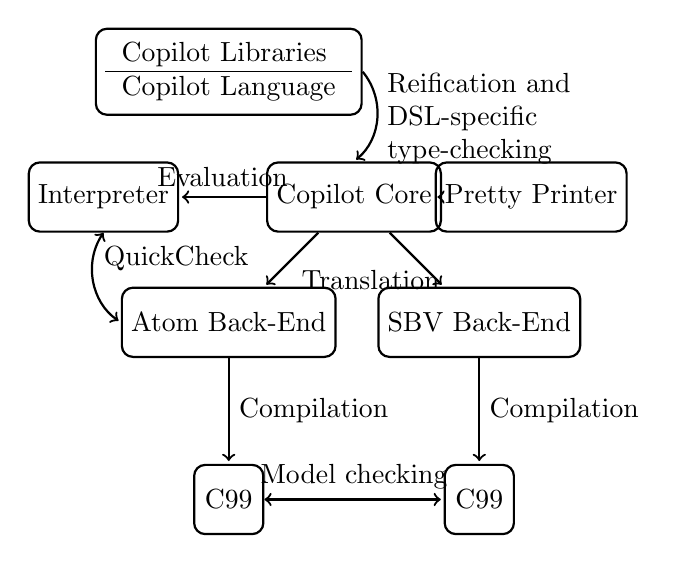
\begin{tikzpicture}[->, node distance=2.25cm, auto, shorten >=1pt, bend angle=45,
      thick]
    \tikzstyle{every state}=[rectangle, rounded corners]

    \node[state]         (Int)            {Interpreter};
    \node[state]         (Lang) [above right of=Int]
         {
           \begin{tabular}[b]{l}
           Copilot Libraries\\ \hline Copilot Language
           \end{tabular}};
    \node[state]         (Core) [below right of=Lang]          {Copilot Core};
    \node[state]         (PP) [right of=Core]          {Pretty Printer};

    \node[state]         (Atom) [below left of=Core]     {Atom Back-End};
    \node[state]         (SBV) [below right of=Core]     {SBV Back-End};
    \node[state]         (C99A) [below of=Atom]     {C99};
    \node[state]         (C99S) [below of=SBV]     {C99};

    \tikzstyle{every node}=[]

    \path %% (Libs) edge              node {0,1,L} (Lang);
    %% edge                 node {1,1,R} (C)
    (Lang) edge   [bend left, anchor=west, text width=2.5cm] node {Reification and DSL-specific type-checking} (Core)
    %% edge                 node {0,1,L} (C)
    (Core) edge              node {Translation} (Atom)
    edge              node {} (SBV)
    edge              node {} (PP)
    edge              node [swap] {Evaluation} (Int)
    (Int) edge              [<->, bend right] node {QuickCheck} (Atom)
    (Atom) edge             node {Compilation} (C99A)
    (SBV) edge             node {Compilation} (C99S)
    (C99A) edge              [<->] node  {Model checking} (C99S);
    
    %% edge [bend left]     node {Translation} (SBV)
    %% (Atom) edge [loop below] node {1,1,R} (D)
    %%     edge                 node {0,1,R} (Libs)
    %% (SBV) edge [bend left]   node {1,0,R} ();
  \end{tikzpicture}
  \caption{The Copilot toolchain.}
  \label{fig:toolchain}
\end{figure}

\todo{confusing}

Copilot's toolchain is depicted in Figure~\ref{fig:toolchain}, which we
highlight here; assurance-relevant aspects of the toolchain are covered in more
detail later.  Copilot is deeply embedded in Haskell.  A Copilot program is
reified (i.e., transformed from a recursive structure into explicit graphs via
observable sharing~\cite{gill}) and then some domain-specific type-checking is
done.  At this point, we have transformed the program into the ``core''
language, an intermediate representation.  The core package contains an
interpreter ($\sim$300~LOCs) as well as a custom QuickCheck engine and test
harness for testing interpreter output against one of the back-ends


%%  and does
%% domain-specific type-checking ($\sim$1200 lines of code or LOCs).


%% The Copilot language package ---  Copilot
%% programs are then translated into a core language ($\sim$900~LOCs).  The core
%% package contains an interpreter ($\sim$300~LOCs) as well as a custom QuickCheck
%% engine and test harness for testing interpreter output against one of the
%% back-ends ($\sim$400~LOCs).  

The back-ends translate a Copilot core program into the language of another
Haskell-hosted EDSL for code generation.  We use the
Atom\footnote{\url{http://hackage.haskell.org/package/atom}, BSD3
  license.}~\cite{atom} and
SBV\footnote{\url{http://hackage.haskell.org/package/sbv}, BSD3 license.}
packages for code generation, both of which generate a subset of C99 embedded
code that is constant-memory and nearly constant-time.  Atom is an EDSL
originally designed by Tom Hawkins at Eaton Corp. for synthesizing real-time
embedded control systems from high-level specifications.  The language provides
scheduling constructs, obviating the need for a real-time operating system when
cooperative scheduling is sufficient.  Symbolic Bit Vectors (SBV) is an EDSL
developed by Levent Erk\"{o}k.  The primary focus of SBV is to express and
reason about bit-level Haskell programs.  In particular, the language provides
tight integration with satisfiability modulo theories (SMT) solvers (e.g.,
Yices~\cite{dutertre}) for automatic proofs and to check for satisfiability.
The EDSL also contains a C-code generator which we use.  Other features of the
language include test-case generation and automated synthesis.

We use the recent Safe Haskell compiler extensions to implement
Copilot~\cite{safe}.  Copilot's language package is explicitly \emph{Trustworthy
  Haskell}, as there is a single instance of {\tt unsafeCoerce} to implement
observable sharing.  Copilot's core language is written in \emph{Safe Haskell}.


A separate package generates a driver for the CBMC
model-checker~\cite{cbmc}, which we use to check the equivalence between the C~code
generated by each back-end.

%--------------------------------------------------------------------------------
\section{Lessons Learned: Quick and Easy Correctness Evidence}
\label{sec:lessons}

In the following, we describe some ``lessons-learned'' in quickly and easily
building assurance into an EDSL compiler.






%--------------------------------------------------------------------------------
\paragraph{Lesson: Turing-complete macros, small, Turing-incomplete languages.}
\label{sec:turing}
C-like languages treat macros as a second-class feature---they are just textual
substitution.  Lisp-like languages take the converse approach, treating macros
as a first-class datatype, so macros are on par with (Turing-complete)
programming.  These are two extremes, but they largely represent the status
of macro programming.

EDSLs, however, treat meta-programming as first-class, and programming as
second-class!  The difference in emphasis of EDSLs is because the embedded
language is a datatype within its host language (we assume a deep-embedding of
the DSL~\cite{gill}).  The difference affects how one programs using an EDSL.
Practically, one spends very little time directly using the operators of the
EDSL itself but rather, one generates EDSL programs using combinators from the
host language.

Embedded system programming, with time and memory constraints, does not require
the full power of a general-purpose Turing-complete language~\cite{CaspiPHP87}.
But a Turing-complete \emph{macro language} affords benefits in code-reuse and
library development.  With an EDSL, one can have his cake and eat it too:
Arbitrarily complex combinators over the EDSL can be written, but then a simple
core language can be reasoned about.

Reasoning about the correctness of sub-Turing-complete languages is easier than
general-purpose languages.  For example, a verifying compiler for a
cryptographic DSL leveraged the ability to automatically generate measures to
formally prove termination of programs written in the language~\cite{mcrypt}.
Conversely, Sassaman~\emph{et~al.} argue that a principal origin of insecurity
in computer systems is due to Turing-complete (or more generally, too powerful)
data-description languages~\cite{turing}.

\begin{figure}[h!t]
  \begin{code}
data Expr a where
  -- Constants
  Const :: Type a -> a -> Expr a
  -- Stream constructors
  Drop  :: Type a -> Int -> Id -> Expr a
  -- Let expressions
  Local :: Type a -> Type b -> Name -> Expr a 
        -> Expr b -> Expr b
  Var   :: Type a -> Name -> Expr a 
  -- Operators
  Op1   :: Op1 a b -> Expr a -> Expr b 
  Op2   :: Op2 a b c -> Expr a -> Expr b -> Expr c
  Op3   :: Op3 a b c d -> Expr a -> Expr b 
        -> Expr c -> Expr d
  -- Externals
  ExternVar   
    :: Type a -> Name -> Maybe [a] -> Expr a 
  ExternFun   
    :: Type a -> Name -> [UExpr] 
    -> Maybe (Expr a) -> Maybe Int -> Expr a
  ExternArray 
    :: Integral a => Type a -> Type b 
    -> Name -> Int -> Expr a -> Maybe [[b]] 
    -> Maybe Int -> Expr b 

-- Untyped streams
data UExpr = forall a. UExpr
  \{ uExprType :: Type a
  , uExprExpr  :: Expr a \}
  \end{code}
\caption{The core Copilot expression language abstract syntax.\label{fig:core}}
\end{figure} 

The core language of Copilot is both small and unpowerful: as noted, only
programs requiring a constant amount of space can be written in Copilot.  In
Figure~\ref{fig:core} is the generalized abstract datatype (GADT)~\cite{gadts}
that is the abstract syntax for Copilot expressions in the core language.  There
are constants, the ``drops'' stream constructor (dropping a finite number of
prefix list elements), let-expressions within Copilot for user-defined
expression sharing, external program inputs, and unary, binary, and ternary
operators.  One final data type, {\tt UExpr} contains existentially-typed
streams that are used in argument lists.  Everything else is syntactic sugar or
specific operators.  (The operational semantics of Copilot, given by an
interpreter function over the {\tt Expr} datatype, is about 200~LOCs.)

Despite the small size of the core language and the lack of computational power,
with Haskell's parametric polymorphism and standard library combinators, we can
enjoy the benefits of code reuse and abstraction in building libraries while
maintaining a terse core language.  For example, in our fault-tolerant voting
library, the Boyer-Moore linear-time Majority Vote algorithm~\cite{mjrty} is
written as a Haskell function that gets expanded at compile-time into a Copilot
program.  Libraries for bounded linear-temporal logic, regular expressions,
bounded folds, bounded scans, etc. are similarly just Copilot macros.

The idea that the macro language can be arbitrarily complex is obvious to the
functional languages community, but it is a disruptive one to the embedded
languages community, particularly for safety-critical systems.  Typical
declarative languages for embedded systems design, like
Lustre~\cite{CaspiPHP87}, are not polymorphic (polymorphism is limited to a
small set of pre-defined operators, like {\tt if-then-else}).

%--------------------------------------------------------------------------------
\paragraph{Lesson: multi-level type-checking.}

Type-checking is the first defense against incorrect programs.  We used a
two-layer approach: let the host language enforce types where possible, and
write a custom checker for type-checking that falls outside of the host
language's type system.  In this way, we rely on Haskell to do most of the heavy
lifting.

We use GADTs to represent both the front-end abstract syntax and the core
language.  The use of parameterized datatypes makes the probability of
unanticipated type-casts low.  There are only two cases during which we escape
Haskell's type system, which may lead to incorrect type-casts.  

The first case is when a back-end pretty-prints C~code.  The correctness of such
code can be determined by inspecting a small number of functions and class
instances.

The second case arises during the translation from the core abstract syntax into
the back-ends, which are themselves EDSLs embedded in Haskell.  Both the core
language and the back-ends make use of polymorphic functions and class
constraints.  As a matter of software engineering, we do not want Copilot's core
functions to be dependent on the classes introduced in the back-ends---doing so
would require modifying functions and datatypes defined in the core with new
class constraints for each time a new back-end is added!

Therefore, we use the ideas of type-safe dynamic typing to translate from the
core language to the back-end languages without relying on compiler extensions
or unsafe functions~\cite{typing}.  The basic idea is to create witness
functions that we pattern-match against.  For example, for the class {\tt
  SymWord} (``Symbolic Word'') in the SBV back-end, we create the following
instance datatype and an instance function mapping Copilot types to {\tt
  SymWord}s:
%
\begin{code}
data SymWordInst a = SymWord a => SymWordInst

symWordInst :: Type a -> SymWordInst a
symWordInst t =
  case t of
    Bool   -> SymWordInst
    Int8   -> SymWordInst
    ...
\end{code}
%
where {\tt Type} is a phantom type containing concrete representations of
Copilot's core types.
%
\begin{code}
data Type :: * -> * where
  Bool    :: Type Bool
  Int8    :: Type Int8
  ...  
\end{code}
%
Then during the translation, we pattern-match.  For example, in translating the
addition operator, we translate from Copilot's {\tt Add} constructor in the core
language to SBV's addition operator {\tt +}:
%
\begin{code}
transBinaryOps op = case op of
  Add t -> case W.symWordInst t of 
             W.SymWordInst ->  (+)
  ...
\end{code}
%
The upshot is that we have created potentially partial translation functions,
but type-incorrect translation is not possible.






%% One challenge with using a polymorphic datatype, such as a GADT, to represent
%% the core language, is in translating the core language into the abstract syntax
%% of the back-ends.  In particular, the back-ends we use 


In addition to type-checking provided by Haskell, we perform a small amount of
custom type-checking ($\sim$250~LOCs).  The two classes of custom type-checking
are (1) causality analysis and (2) type-checking external variables (arrays and
functions).  Causality analysis ensures that stream dependencies are evaluated
strictly.  Strict dependencies are necessary when we are sampling variable
values in real-time from the external world.  For example, the following Copilot
stream equations fail type-checking since {\tt y} initially depends on values
from the variable {\tt x} before any values have been generated:
%
\begin{code}
x :: Stream Word8
x = extern "ext" Nothing
y = drop 2 x 
\end{code}
%
We also check at compile-time that streams are productive; for example, the
stream definition {\tt x = x} fails type-checking.

In addition, external variables are just strings with associated types.
Therefore, we must check that the same string is not given two different types
or declared to be of two different kinds of symbols (e.g,. a global variable
vs. a function symbol).  For example, the following two expressions, if they
appear in the same Copilot program, fail type-checking:
%
\begin{code}
x :: Stream Word8
x = extern "ext" Nothing

y :: Stream Word16
y = extern "ext" Nothing
\end{code}



%--------------------------------------------------------------------------------
\paragraph{Lesson: cheap front-end/back-end testing.}

QuickCheck~\cite{qc} testing is so easy to implement and so effective that no
EDSL compiler should be without it.  QuickCheck can of course be used for unit
testing during compiler development, but we use it to generate regression tests
for the semantics of the EDSL by comparing the output of the interpreter against
the Atom back-end (we plan to implement QuickCheck testing against the SBV
back-end in the future).

We generate a stand-alone executable that for a user-specified number of iterations,
\begin{enumerate}
\item generates a random Copilot program,
\item compiles the Copilot program to C,
\item generates a {\tt driver.c} file containing a {\tt main} function as well
  as values for external variables,
\item compiles and links an executable (using \emph{gcc}),
\item executes the program,
\item and compares its output to the output from the Copilot interpreter.
\end{enumerate}

\noindent
Weights can be set to determine the frequency of generating the various Copilot
language constructs and streams of different types.  

There are at least two approaches to generating type-correct programs.  First,
we can generate random programs, then filter ill-typed programs using the
type-checker.  Second, we can generate type-correct programs directly.  We take
the second approach.  Generating type-correct programs is not difficult in our
case: as described already, because Copilot's abstract syntax is parameterized
by Haskell type variables, type-correct expression generation is
straight-forward.  We need only to ensure the small number of domain-specific
type rules are also satisfied.

The benefit of generating type-correct programs directly is that if the
generator is implemented correctly, every generated program is type-correct and
will be tested.  The danger, however, is that the generator may be too strict,
omitting some type-correct programs from being generated and tested.

With the standard options, we generate, compile, test and pretty-print to
standard output about 1,000 programs per minute.  It is easy to let the
QuickCheck test generator run continuously on a server, generating some million
and a half programs per day (in practice, bugs, if present, tend to appear after
just 10s or 100s of generated programs).  The kinds of bugs we have caught
include forgotten witness for the Atom back-end and the ``out-of-order'' bugs in
which the interpreter output stream values \emph{before} sampling variables.  A
``non-bug'' we discovered was disagreement on floating-point values between
GHC's runtime system (executing the interpreter) and \emph{libc}.  We solved
this problem by just checking that floating point values are within some small
constant range, noting that pathological cases may cause differences outside of
a constant range without violating the IEEE floating-point standard.

%--------------------------------------------------------------------------------
\paragraph{Lesson: cheap back-end proofs.}
The verified compiler approach assumes that the compiler itself is within the
\emph{trusted computing base} (TCB)---the software that must be trusted to be
correct.  Consequently, it requires a monolithic approach to verification in
which the compiler is verified.  But what if the compiler can be removed from
the TCB?  Doing so can reduce the difficulty of providing assurance evidence.

This is our motivation for a proof approach of the back-ends.  Recalling
Figure~\ref{fig:toolchain}, Copilot has two back-ends that generate C.  We
leverage the open-source model-checker CBMC to prove the equivalence of the code generated by each
back-end~\cite{cbmc}.  CBMC uses C as its
specification language.  In our work, we use CBMC.  CBMC can prove memory-safety
properties, such as no division by zero, no not-a-number floating-point errors,
and no array out-of-bound indexes.  It can also prove arbitrary propositional
formulas given in the body of {\tt assert()} functions.

To prove equivalence between the two back-end outputs, we automatically generate
a driver program that executes both back-ends for one step, compares their
outputs, takes another step, compares their outputs, and so on for a
user-specified number of iterations.  The generated driver is
of the form
%
\begin{code}
for (i = 0; i < RNDS; i++) \{
  sampleExterns();
  atom_step();
  sbv_step();
  assert(   atomStr_0 == sbvStr_0 
         && atomStr_1 == sbvStr_1  
         && ... );
\}
\end{code}
%
For sampled variables (arrays, functions), we use CBMC's built-in model of
nondeterminism to model arbitrary inputs to Copilot programs.  CBMC proves the
two programs are memory-safe and have equivalent semantics for a finite number
of user-specified iterations ({\tt RNDS}).  

Model-checking works ``out of the box'' in our case because both back-ends
generate simple code (e.g., no non-linear pointer arithmetic, no function
pointers, no loops) in the state-update functions.  This use of formal methods
emphasizes the lesson about simple, Turing-incomplete languages from
Section~\ref{sec:turing}.

A proof of correspondence on the C code reduces the trust required in the Atom
and SBV back-ends.  Assuming the model-checker is sound, incorrectly-generated
code will be claimed to be equivalent only if bugs with the same effects appear
in both back-ends.  In addition, memory-safety errors, even if they appear
simultaneously in both programs, will be caught.

That said, one must still trust the C compiler---CompCert~\cite{leroy} would be
a good point in this case.  Furthermore, Copilot programs are expected to be
executed forever (i.e., they are programs over infinite streams), which mimics
the behavior of embedded software.  CBMC symbolically unrolls programs either
completely if possible or to a user-specified depth; it does not perform an
inductive proof, so currently, we only show equivalence up to a user-set bound
({\tt RNDS} in the code-snippet above).  Using a model-checker with induction
(e.g., $k$-induction via SAT~\cite{tinelli}) would strengthen the
assurance case.  Finally, note that this use of model-checking takes the
verifying rather than verified-compiler approach: model-checking is done for
\emph{each} program compiled.

The kinds of bugs we have caught mostly include incorrect ordering of
functions in the generated C (e.g., sampling external values after computing
next-state values for streams).  Because we do not yet have a
QuickCheck testing infrastructure between the interpreter and the SBV back-end,
we get a transitive argument that the SBV back-end is equivalent to the Atom
back-end, which has evidence of matching the interpreter through the use of
QuickCheck.  From an evidence perspective, model-checking the back-ends reduces
the required trust in the Haskell compiler/interpreter, since we check the generated
artifacts.  Ideally, we would have the power of an EDSL without having to trust
the runtime system of the host language.


%--------------------------------------------------------------------------------

\paragraph{Lesson: a unified host language.}
Our last lesson is one obvious to the functional programming community, but
novel in safety-critical languages.  EDSLs are intrinsically immune to whole classes of
potential compiler bugs.  For example, because a separate parser, lexer,
tokenizer, etc. are not necessary, EDSLs do not suffer from these front-end
bugs.  This assumes that the host language's front-end does not contain bugs,
which for a stable well-used host language, is more likely than for a new DSL
front-end.  

We enjoyed two other advantages.  First, translating between EDSLs in the same
host language was type-safe and relatively easy since the two back-ends we use were
existing EDSLs.  Translating from Copilot into a back-end is a matter of
converting from one abstract syntax datatype into another, never leaving the host
language.  

Second, the host language serves as more than a macro language: it serves as a
partial build system.  For example, consider the case of generating distributed
Copilot programs to be run on networked processors, where we want to
parameterize inputs based on the processor identifier.  With an EDSL, this is no
more difficult than parameterizing the {\tt compile} function.  In our
experiments with NASA, we did just this to build fault-tolerant
monitors~\cite{pike-rv-11}.


%--------------------------------------------------------------------------------
\section{Related Work}
\label{sec:related}

Our experience report builds on research in disparate fields including
functional programming and EDSL design, compiler verification, and embedded
safety-critical languages.  In this section, we provide just a few pointers into
the literature that inspired us.

Some might believe that compilers are generally bug-free (even if specific
programs are buggy).  Work at the University of Utah has dispelled this
myth~\cite{rehger}, having uncovered hundreds of bugs in C compilers like
\emph{gcc}, \emph{clang}, and even the (unverified) front-end of the CompCert
compiler~\cite{leroy}.  Compiler verification is still important.  Our work does
not address C compilation directly, but it does reduce the risk of encountering
bugs in C compilers by constraining the language to a small subset of
well-defined C.

%% EDSLs have long been proposed as a method for easing the difficulty of writing
%% programs 

FeldSpar is an EDSL in Haskell designed for digital signal processing designed
by Ericsson and Chalmers University~\cite{feldspar1}.  FeldSpar's architecture
and implementation is similar to Copilot's and could integrate the assurance
approaches we have described.  Researchers at the University of Minnesota have
also built a family of DSLs tailored for safety-critical embedded system
modeling~\cite{mats}.  The host language was designed so that new DSLs can be
specified using attribute grammars.  It appears the purpose of the language is
primarily for modeling, so the work does not address compilation, and
consequently does not address compiler correctness issues.  Finally,
Filet-o-Fish is a related DSLs framework for operating system
development~\cite{fof}.  The authors emphasize compiler assurance as we do, also
using an interpreter to provide an operational semantics and using QuickCheck
for testing.

An alternative to the EDSL approach is to take a functional language and augment
it with sufficient evidence to be used directly in safety-critical contexts,
such as avionics development.  A consortium did just that with OCaml, rewriting
the SCADE code generator~\cite{ocaml}.  Qualifying the software required
substantially reducing OCaml's runtime system and garbage collector, extensive
testing, and providing ``traceability'' of requirements.  From a formal
verification perspective, the requirements are lightweight (the main direct
evidence for correctness is testing).


%%  \thispagestyle{fancy}
%% \chead{\small Appears in the proceedings of the {\em 2nd International
%%     Conference on Runtime Verification} (RV 2011).}

%--------------------------------------------------------------------------------
\section{Conclusions}
\label{sec:conclusions}

Despite our experience, EDSLs are not a panacea.  Copilot suffers the same
problems that many EDSL implementations do.  Error messages from the Haskell
compiler are not domain-specific.  There is no graphical development environment
(common in embedded systems development).  Large Haskell expressions are easy to
generate, which can be expensive to interpret or compile.  Copilot does not
currently have a highly-optimizing back-end.

Regarding our approach to compiler assurance, there are some weaknesses.  First,
since the interpreter and back-ends are built on the core language, bugs in
translation from the front-end will affect all the targets.  While QuickCheck
tests the executables against the interpreter, the model-checker only proves
properties about (its interpretation of) the C source semantics.  CompCert would
obviously be a good choice to compile C, then.  Finally, as noted in the
introduction, we have focused here on evidence of correct compilation, but our
implementation does not necessarily help ensure a specific program meets its
specification.  These shortcomings point to future research efforts.

In summary we hoped to make two points in this report: first, that EDSLs are a
viable approach for building high-assurance compilers, and second, that strong
evidence can be generated with little work or expertise.  With the EDSL, you do
not have to write your own front-end, most type-checking is done for you, and
today's off-the-shelf model-checkers are capable of checking real programs.

But don't take our word for it; do-it-yourself.

\acks 

This work was supported by NASA Contract NNL08AD13T.  We wish to especially
thank the following individuals for advice on our work: Ben Di~Vito, Paul Miner,
Eric Cooper, Joe Hurd, and Aaron Tomb.  Robin Morisset worked on an
earlier version of Copilot.  Nis Wegmann and Sebastian Niller completed this
work while they were visiting researchers at the National Institute of
Aerospace.   


%% \balancecolumns

\bibliographystyle{abbrvnat}
\bibliography{paper}

\end{document}

